\documentclass[11pt,letterpaper]{article}
\usepackage{fullpage}
\usepackage{multicol}
\usepackage{amsmath}
\usepackage{amsfonts}
\usepackage{amssymb}
%\usepackage{pstricks, pst-node, pst-plot}

\ifx\pdfoutput\undefined
% we are running LaTeX, not pdflatex
\usepackage{graphicx}
\else
% we are running pdflatex, so convert .eps files to .pdf
\usepackage[pdftex]{graphicx}
\usepackage{epstopdf}
\fi

\newcommand{\ds}{\displaystyle}
\newcommand{\bv}{\mathbf}
\newcommand{\lv}{\langle}
\newcommand{\rv}{\rangle}

\begin{document}
\flushleft
\begin{multicols}{2}

\begin{large}\textbf{Math 116 Quiz 6: $\oint$ 4.8, 8.3, 7.7-7.8 \\
Tue 6 Nov 2012}\end{large}

\textbf{Name:  }\underline{\hspace{4pc}{\bf SOLUTIONS}\hspace{4pc}}

\vspace{.5in}

\end{multicols}

\pagestyle{empty}


\flushleft

You have 45 minutes to complete this quiz.  Eyes on your own paper and good luck!

\begin{enumerate}
\item  \textbf{Definitions/Concepts.}
\begin{enumerate}
\item (3 pts) {\bf Parametrizing a Line:} Given $\frac{dx}{dt}=a$ and $\frac{dy}{dt}=b$, a line passing through the point $(x_0,y_0)$ has the following parametric equations:
\begin{align*}
x(t) &= x_0+at\hspace{160pt}\\
y(t) &= y_0+bt
\end{align*}
The non-parametric equation for the same line is given by:
\[y-y_0=\frac{b}{a}(x-x_0)\]
%\vspace{3pc}
\item (1 pt) Given polar coordinates $(r,\theta)$, the same point in Cartesian coordinates is 
\begin{align*}
x &= r\cos\theta\hspace{170pt}\\
y &= r\sin\theta
\end{align*}
\end{enumerate}

 
\item \textbf{Questions/Problems.} {\it (from Fall 2011 Exam 2)} Members of the recruitment committee for the Mars University (MU) chapter of the fraternity Epsilon Rho Rho (ERR) are designing a pledge pin to distribute during Rush Week.  The pin takes the shape of a cardioid with a circular hole in it.  The cardioid is given by a polar equation of the form $r_1=a+b\cos\,\theta$, while the circular hole has the polar equation $r_2=\cos\,\theta$.  The pin is pictured below, where the $x$- and $y$-axes are measured in inches.
\smallskip
\begin{center}
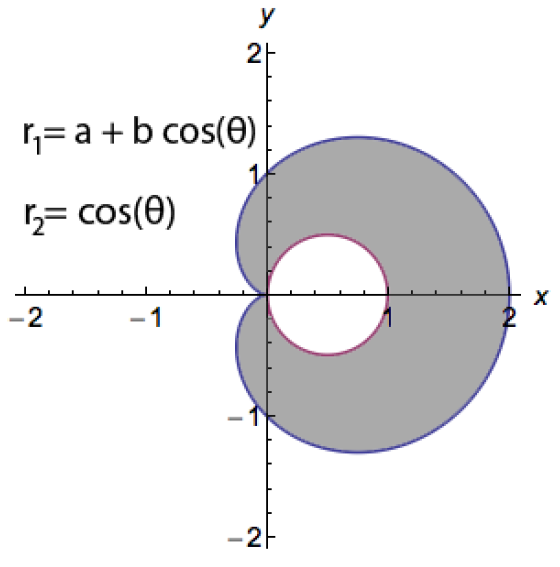
\includegraphics[width=.35\textwidth]{quiz6pic.png}
\end{center}
\begin{enumerate}
\item (5 pts) The committee plans on coating one side of the pin in gold plating, which costs 3 dollars per square inch.  Give an expression representing the cost to plate one face of the pin in gold.  Your answer may involve integrals and the constants $a$ and $b$.

{\it -see the solution posted on the course website -}
\vspace{10pc}
\item (3 pts) Find $a$ and $b$.

{\it -see the solution posted on the course website -}
\vspace{9pc}
\end{enumerate}

\vspace{1pc}
%\hfill{\bf MORE QUIZ ON THE BACK --\textgreater}

\item \textbf{Computations/Algebra.} (2 pts)  Determine if the following integrals converge or diverge.  If an integral converges, compute the value to which it converges.  If an integral diverges, you must explain why.  \begin{enumerate}
\item $\int_{-2}^2\frac{dx}{x^2}=$
\[\int_{-2}^0\frac{dx}{x^2}+\int_0^2\frac{dx}{x^2},\]
since the integrand diverges when $x=0$.  We must take limits in order to evaluate, so we get
\begin{align*}
\lim_{b\to 0^-}\int_{-2}^b\frac{dx}{x^2}+\lim_{a\to 0^+}\int_a^2\frac{dx}{x^2} &= \lim_{b\to 0^-}\left.\frac{-1}{x}\right|_{-2}^b+\lim_{a\to 0^+}\left.\frac{-1}{x}\right|_a^2 \\
&= \lim_{b\to 0^-}\left(\frac{-1}{b}-\frac{-1}{-2}\right)+\lim_{a\to 0^+}\left(\frac{-1}{a}-\frac{-1}{2}\right) \\
&= \lim_{b\to 0^-}\left(\frac{-1}{b}-\frac{1}{2}\right)+\lim_{a\to 0^+}\left(\frac{-1}{a}+\frac{1}{2}\right) \\
&= \infty
\end{align*}
and so the integral diverges.
\vspace{0.5pc}
\item $\int_{-1}^2\frac{dx}{\sqrt{2-x}}=$
\begin{align*}
\lim_{b\to 2^-}\int_{-1}^b\frac{dx}{\sqrt{2-x}} &=\lim_{b\to 2^-}\left.-2\sqrt{2-x}\,\right|_{-1}^b \\
&= -2\sqrt{2-2}-\left(-2\sqrt{2-(-1)}\right) \\
&= 2\sqrt{3}
\end{align*}
%\vspace{10pc}
\item $\int_{10}^{\infty}\frac{5+2\sin\,4\theta}{\theta}d\theta=$

Before integrating, notice the sine function is bounded between $-1$ and $1$.  So for $\theta>>0$ (the $>>$ sign means ``for $\theta$ sufficiently large"), we have the inequality
\[\frac{1}{\theta}\leq\frac{3}{\theta}\leq\frac{5+2\sin{4\theta}}{\theta}\leq\frac{7}{\theta},\]
but in particular, 
\[\int_{10}^{\infty}\frac{1}{\theta}\,d\theta=\int_1^{\infty}\frac{1}{\theta}d\,\theta-\int_1^{10}\frac{1}{\theta}d\,\theta\]
and the right hand side diverges.  Therefore the integral $\int_{10}^{\infty}\frac{5+2\sin\,4\theta}{\theta}d\theta$ also diverges.
\vspace{0.5pc}
\item $\int_1^{\infty}\frac{x}{1+x}dx=$

To conclude divergence, it is not enough to say the function $\frac{x}{1+x}$ behaves like the constant function $1$ for $x>>0$.  However, we can set up an explicit inequality.  Notice
\[\frac{1}{2}=\frac{x}{x+x}\leq\frac{x}{1+x}\]
for $x>>0$.  Integrating $\frac{1}{2}$ is the same as integrating the function $1$ and then multiplying the result by $\frac{1}{2}$; i.e., 
\[\int_1^{\infty}\frac{1}{2}\,dx=\frac{1}{2}\int_1^{\infty}1\,dx,\]
which diverges.  Therefore the original integral $\int_1^{\infty}\frac{x}{1+x}dx$ diverges.
\end{enumerate}

\end{enumerate}

\end{document}


